%% A minimal LaTeX preamble
%% Some packates are needed to implement
%% Asciidoc features

\documentclass[12pt,twoside]{article}
\usepackage[brazilian]{babel}
\usepackage[left=3.00cm, right=2.00cm, top=3.00cm, bottom=2.00cm]{geometry}                % See geometry.pdf to learn the layout options. There are lots.
%\geometry{letterpaper}               % ... or a4paper or a5paper or ...
%\geometry{landscape}                % Activate for for rotated page geometry
%\usepackage[parfill]{parskip}       % Activate to begin paragraphs with an empty line rather than an indent

\usepackage{tcolorbox}
\usepackage{lipsum}

\usepackage{epstopdf}
\usepackage{color}
% \usepackage[usenames, dvipsnames]{color}
% \usepackage{alltt}


\usepackage{amssymb}
% \usepackage{amsmath}
\usepackage{amsthm}
\usepackage{cancel}
\usepackage[version=3]{mhchem}


% Needed to properly typeset
% standard unicode characters:
%
\RequirePackage{fix-cm}
\usepackage{fontspec}
\usepackage[Latin,Greek]{ucharclasses}
% NOTE: you must also use xelatex
% as the typesetting engine


% \usepackage{fontspec}
% \usepackage{polyglossia}
% \setmainlanguage{en}

\usepackage{hyperref}
\hypersetup{
    colorlinks=true,
    linkcolor=blue,
    filecolor=magenta,
    urlcolor=blue,
}

\usepackage{fancyhdr}
\pagestyle{fancy}
%\renewcommand{\headrulewidth}{1pt} % retirando linha
%\renewcommand{\footrulewidth}{1pt} % colocando linha

\usepackage{graphicx}
\usepackage{wrapfig}
\graphicspath{ {images/} }
\DeclareGraphicsExtensions{.png, .jpg, jpeg, .pdf}

%% \DeclareGraphicsRule{.tif}{png}{.png}{`convert #1 `dirname #1`/`basename #1 .tif`.png}
%% Asciidoc TeX Macros %%


% \pagecolor{black}
%%%%%%%%%%%%


% Needed for Asciidoc

\newcommand{\admonition}[2]{\textbf{#1}: {#2}}
\newcommand{\rolered}[1]{ \textcolor{red}{#1} }
\newcommand{\roleblue}[1]{ \textcolor{blue}{#1} }

\newtheorem{theorem}{Theorem}
\newtheorem{proposition}{Proposition}
\newtheorem{corollary}{Corollary}
\newtheorem{lemma}{Lemma}
\newtheorem{definition}{Definition}
\newtheorem{conjecture}{Conjecture}
\newtheorem{problem}{Problem}
\newtheorem{exercise}{Exercise}
\newtheorem{example}{Example}
\newtheorem{note}{Note}
\newtheorem{joke}{Joke}
\newtheorem{objection}{Objection}





%%%%%%%%%%%%%%%%%%%%%%%%%%%%%%%%%%%%%%%%%%%%%%%%%%%%%%%

%  Extended quote environment with author

\renewenvironment{quotation}
{   \leftskip 4em \begin{em} }
{\end{em}\par }

\def\signed#1{{\leavevmode\unskip\nobreak\hfil\penalty50\hskip2em
  \hbox{}\nobreak\hfil\raise-3pt\hbox{(#1)}%
  \parfillskip=0pt \finalhyphendemerits=0 \endgraf}}


\newsavebox\mybox

\newenvironment{aquote}[1]
  {\savebox\mybox{#1}\begin{quotation}}
  {\signed{\usebox\mybox}\end{quotation}}

\newenvironment{tquote}[1]
  {  {\bf #1} \begin{quotation} \\ }
  { \end{quotation} }

%% BOXES: http://tex.stackexchange.com/questions/83930/what-are-the-different-kinds-of-boxes-in-latex
%% ENVIRONMENTS: https://www.sharelatex.com/learn/Environments

\newenvironment{asciidocbox}
  {\leftskip6em\rightskip6em\par}
  {\par}

\newenvironment{titledasciidocbox}[1]
  {\leftskip6em\rightskip6em\par{\bf #1}\vskip-0.6em\par}
  {\par}



%%%%%%%%%%%%%%%%%%%%%%%%%%%%%%%%%%%%%%%%%%%%%%%%%%%%%%%%

%% http://texblog.org/tag/rightskip/


\newenvironment{preamble}
  {}
  {}

%% http://tex.stackexchange.com/questions/99809/box-or-sidebar-for-additional-text
%%
\newenvironment{sidebar}[1][r]
  {\wrapfigure{#1}{0.5\textwidth}\tcolorbox}
  {\endtcolorbox\endwrapfigure}


%%%%%%%%%%

\newenvironment{comment*}
  {\leftskip6em\rightskip6em\par}
  {\par}

  \newenvironment{remark*}
  {\leftskip6em\rightskip6em\par}
  {\par}


%% Dummy environment for testing:

\newenvironment{foo}
  {\bf Foo.\ }
  {}


\newenvironment{foo*}
  {\bf Foo.\ }
  {}


\newenvironment{click}
  {\bf Click.\ }
  {}

\newenvironment{click*}
  {\bf Click.\ }
  {}

\newenvironment{resposta}
{\bf Resposta:\\ }
{}

\newenvironment{resposta*}
{\bf Resposta:\\ }
{}


\newenvironment{remark}
  {\bf Remark.\ }
  {}

\newenvironment{capsule}
  {\leftskip10em\par}
  {\par}

%%%%%%%%%%%%%%%%%%%%%%%%%%%%%%%%%%%%%%%%%%%%%%%%%%%%%

%% Style

\parindent0pt
\parskip8pt
%% User Macros %%
%% Front Matter %%

\title{Propagação de Calor}
\author{Jefferson Rodrigues de Oliveira}
\date{}


%% Begin Document %%

\begin{document}
\maketitle
\begin{center}
	E-mail: \href{mailto:jefferson.oliveira@ifes.edu.br}{jefferson.oliveira@ifes.edu.br} \\
	\vspace{1cm}
	\footnotesize{Atualizado em: \today}
\end{center}
\tableofcontents
\newpage
\hypertarget{x-introdução}{\section{Introdução}}
Caro aluno, se você encontrar qualquer tipo de \textbf{erro} neste \textbf{material didático}, envie-me um \textbf{e-mail}, com o seguinte assunto: \textbf{erro no material didático}. Identifique e explique no corpo do seu e-mail o erro apontado. Ficarei \textbf{bastante grato} pelo seu contato!


No capítulo anterior, estudamos \textbf{as mudanças e os diagramas de fase}. Percebemos que existem três estados fundamentais da matéria: \textbf{sólido}, \textbf{líquido} e \textbf{gasoso}.


Você deve ter percebido que a quantidade de calor que está associada com a mudança de fase, sem ocorrer mudança de temperatura, é denominada de \textbf{calor latente}. Matematicamente, pode ser expressa como:\[Q=m\cdot L\]


Você também aprendeu sobre as curvas de aquecimento ou resfriamento. Para \textbf{substâncias puras}, existe um \textbf{valor fixo} para o calor latente de fusão (ou liquefação) e calor latente de vaporização (ou condensação).


Lembra do \textbf{comportamento anômalo da água}? Então, em geral, a maioria das substâncias aumentam de volume na \textbf{fusão}, enquanto a \textbf{água}, \textbf{diminui de volume}.


Enfim, você percebeu que existe um ponto específico no diagrama de fases chamado de \textbf{ponto triplo}, neste ponto há uma \textbf{coexistência das três fases}. No caso da \textbf{água}, por exemplo, é preciso que a temperatura seja de $273,16\;K$, cerca de \textbf{$0,01\;°C$}, e que a pressão seja de \textbf{$611\;Pa$}. \textbf{Nenhuma} outra \textbf{combinação} de \textbf{pressão e temperatura} é capaz de promover a \textbf{coexistência} dos estados físicos da água. Já o \textbf{ponto crítico} é de aproximadamente \textbf{$374\;°C$}, isso indica que, para \textbf{temperaturas menores} que essas, a água líquida até pode evaporar, no entanto, \textbf{não se comportará como um gás, mas como vapor}.


\begin{figure}[ht]{}
\centering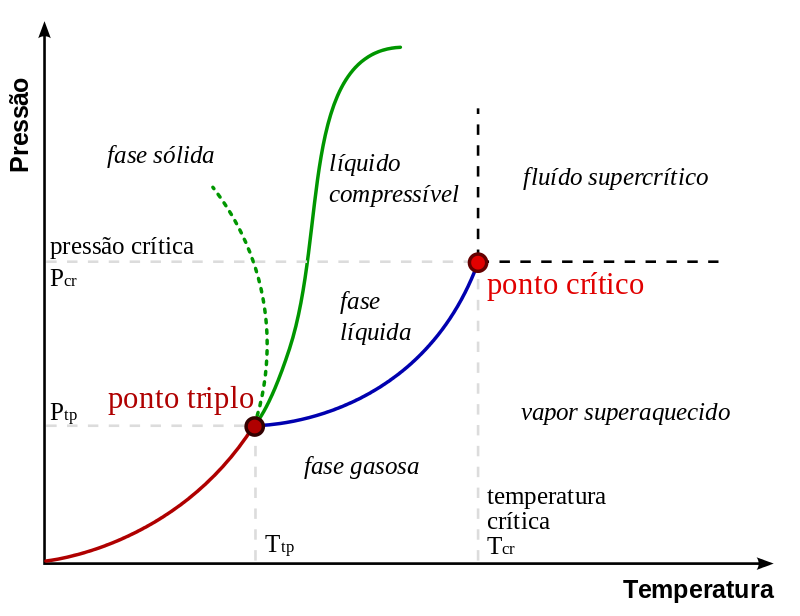
\includegraphics[width=2.5truein]{ponto-triplo.png}
\caption{Diagrama de fases. Fonte: Wikimedia}

\end{figure}

\hypertarget{x-objetivos}{\section{Objetivos}}
Listo aqui abaixo \textbf{os principais objetivos que você deve alcançar} ao estudar este capítulo:


\begin{itemize}

\item \textbf{Saber} que a sensação térmica está ligada à taxa de  transferência de calor e, portanto, à condutividade térmica do material ao qual o individuo está em contato.

\item \textbf{Compreender} que a maioria dos fluidos, quando aquecidos, se expande, diminuindo sua densidade, e sobe devido ao empuxo.

\item \textbf{Compreender} o que são correntes de convecção.

\item \textbf{Exemplificar} situações do cotidiano envolvendo transferência de energia por radiação.

\end{itemize}


\hypertarget{x-considerações-iniciais}{\section{Considerações Iniciais}}
Está preparado para iniciar os estudos dos processos de \textbf{propagação de calor}? Então vamos começar! Você já aprendeu que o \textbf{calor} é um tipo de \textbf{energia em trânsito}, e que pode de forma espontânea, mudar de uma região de \textbf{maior temperatura}, para uma região de \textbf{menor temperatura}. Este processo pode acontecer de três formas: \textbf{condução}, \textbf{convecção} e \textbf{irradiação}.


Para estes três tipos de propagação, podemos definir o \textbf{fluxo de calor ($\phi$)}. O fluxo de calor (fluxo térmico ou corrente térmica) através da superfície é dado pela relação entre a \textbf{quantidade de calor ($Q$)} que atravessa a superfície e o \textbf{intervalo de tempo ($\Delta t$)} decorrido. Sendo assim, matematicamente: \[\phi=\dfrac{Q}{\Delta t}\]


A unidade \textbf{usual} do fluxo de calor é \textbf{$cal/s$} ou \textbf{$kcal/s$}. Mas no Sistema Internacional de Unidades (\textbf{SI}), a unidade é o watt (\textbf{W}), que corresponde ao joule por segundo (\textbf{J/s}).


\textbf{Exercício Resolvido 1}


Uma placa é atravessada por uma quantidade de calor igual a $6,0\times 10^{3}\;cal$ em um intervalo de tempo de $5$ minutos. Determine o fluxo de calor através dessa placa expressa em watt. Considere $1\;cal=4\;J$.


\begin{resposta*}
{\it Aqui, primeiramente devemos transformar a quantidade de calor de calorias ($cal$) para joules ($J$): \[6,0\times 10^{3}\;\cancel{cal} \cdot 4\;\frac{J}{\cancel{cal}} = 240000\;J\]

Agora, precisamos transformar o intervalo de tempo de minutos para segundos: \[5\;\cancel{min}\cdot 60\;\frac{s}{\cancel{min}} = 300\;s\]

Por fim, utilizando a fórmula do fluxo de calor, obteremos o seguinte: \[\phi = \dfrac{24000}{300}\;J/s\]

Como $1\;J/s=1\;W$, então o fluxo de calor será: \[\boxed{\phi = 80\;W}\]}
\end{resposta*}

Fácil, não é mesmo? Mas vamos avançar nossos estudos para a \textbf{condução térmica} e a \textbf{Lei de Fourier}.


\hypertarget{x-condução-de-calor}{\section{Condução de Calor}}
A \textbf{condução} é o processo de propagação de calor no qual a energia térmica passa de \textbf{partícula para partícula} de um meio. É necessário destacar que a condução \textbf{precisa de um meio material}, ou seja, \textbf{não} ocorre no \textbf{vácuo}.


\begin{figure}[ht]{}
\centering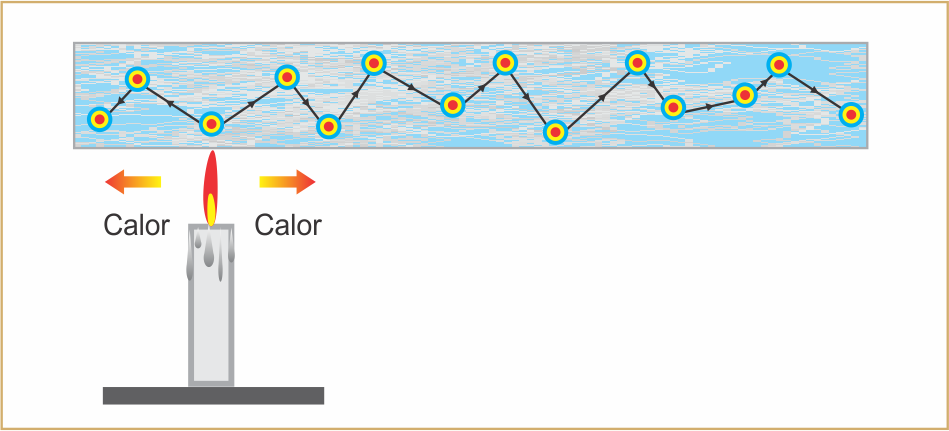
\includegraphics[width=2.5truein]{conducao.png}
\caption{Condução térmica. Fonte: blog os fundamentos da física}

\end{figure}

\hypertarget{x-lei-de-fourier}{\subsection{Lei de Fourier}}
Em \textbf{regime estacionário} (ou permanente), o fluxo de calor por condução num material homogêneo é diretamente proporcional à área da seção transversal atravessada (\textbf{A}) e à diferença de temperatura entre os extremos (\textbf{$\theta_{2}-\theta_{1}$}), e inversamente proporcional à espessura da camada considerada (\textbf{e}).


\begin{figure}[ht]{}
\centering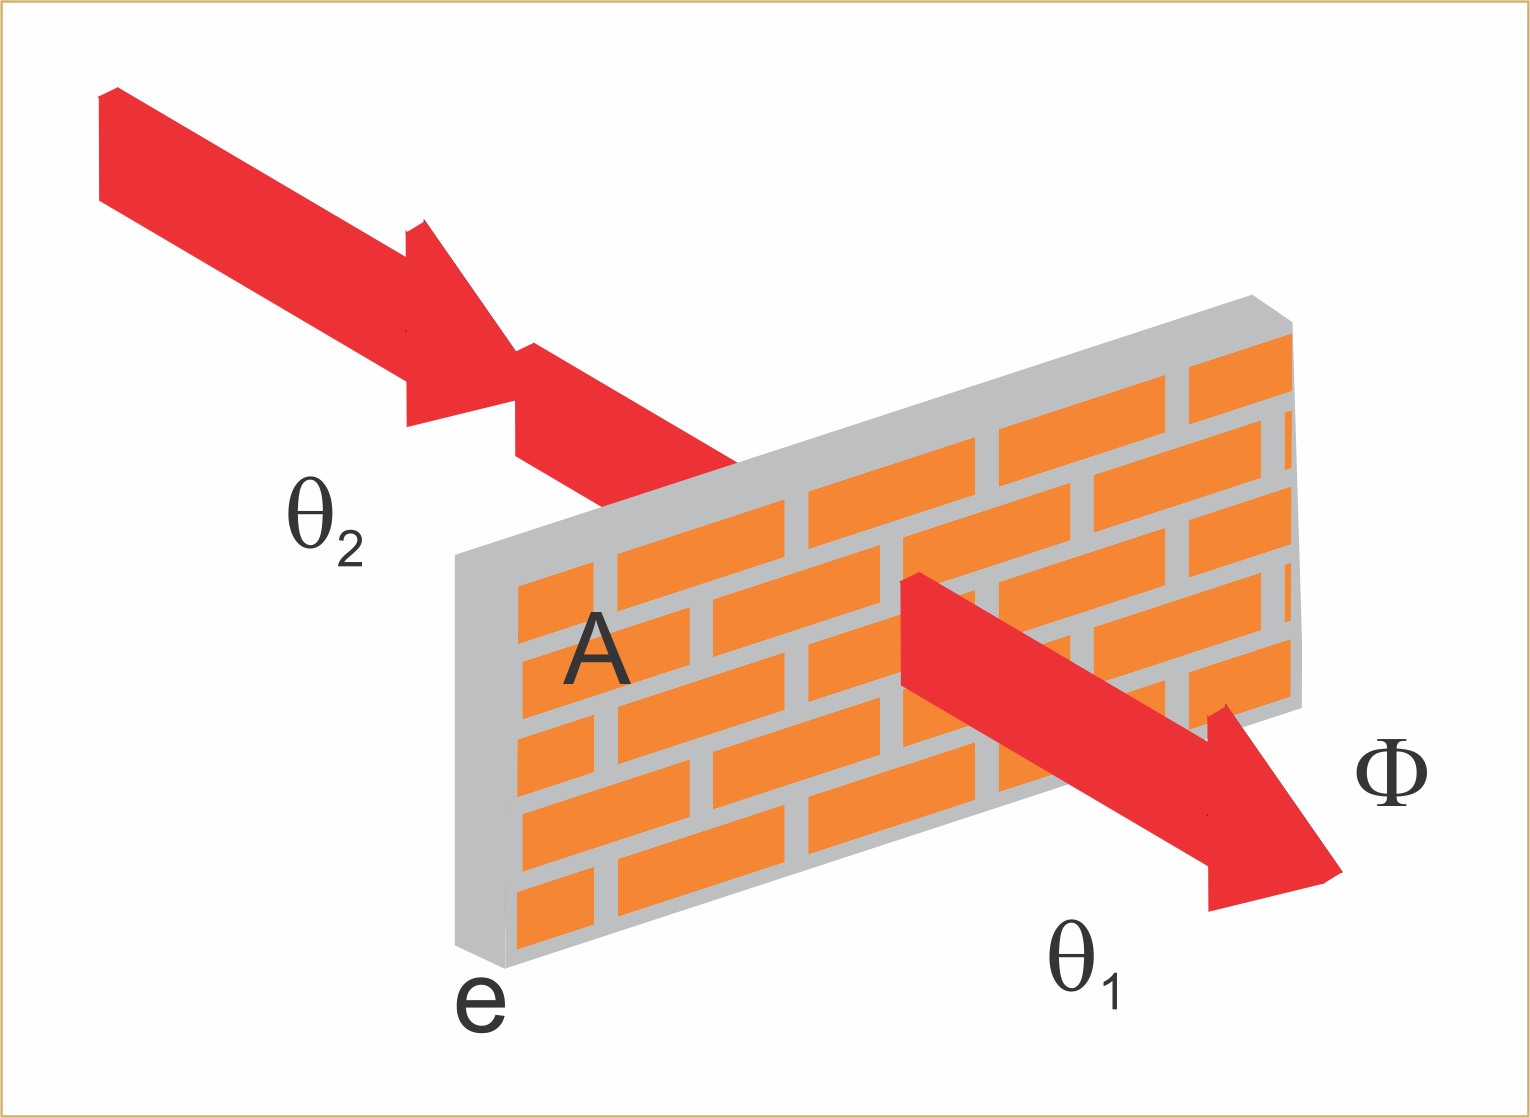
\includegraphics[width=2.5truein]{parede.png}
\caption{Condução através de uma parede. Fonte: blog os fundamentos da física}

\end{figure}

Matematicamente, a \textbf{Lei de Fourier} é expressa da seguinte forma: \[\phi=\dfrac{K\cdot A\cdot(\theta_{2}-\theta_{1})}{e}\]


A constante de proporcionalidade \textbf{K} depende da natureza do material, sendo conhecida como \textbf{coeficiente de condutibilidade térmica}. Seu valor é \textbf{elevado} para \textbf{bons condutores} de calor (condutores térmicos),como os metais, mas \textbf{baixo} para os \textbf{isolantes} térmicos. Exemplos:


\begin{center}
\begin{tabular}{|c|c|}
\hline
\textbf{Material} & \textbf{K [cal/(s.cm.°C)]} \\ 
Prata & $0,99$ \\ 
Alumínio & $0,50$ \\ 
Ferro & $0,16$ \\ 
Água & $0,0014$ \\ 
Lã & $0,0000086$ \\ 
Ar seco & $0,0000061$ \\ 
\hline
\end{tabular}
\end{center}

Aqui você pode perceber que, de uma forma geral, os \textbf{metais} são \textbf{bons condutores} térmicos.


\textbf{Exercício Resolvido 2}


Uma barra de alumínio, com coeficiente de condutibilidade térmica $0,5\;cal/(s.cm.°C)$, está em contato numa extremidade com gelo em fusão e na outra com vapor de água em ebulição sob pressão normal. Seu comprimento é $25\;cm$ e a secção transversal tem $5\;cm^{2}$ de área. Sendo a barra isolada lateralmente e dados o calor latente de fusão do gelo $80\;cal/g$ e o calor latente de vaporização da água $540\;cal/g$, determine:


a) O fluxo de calor em $cal/s$. \\
b) A massa de gelo, em gramas, que se funde em meia hora. \\
c) A massa de vapor, em gramas, que se condensa no mesmo tempo. \\
d) A temperatura numa seção da barra a $5\;cm$ da extremidade fria.


\begin{resposta*}
{\it a) Para encontrar o fluxo de calor atravessado pela barra, precisaremos utilizar a Lei de Fourier:

\begin{align*}
\phi &= \dfrac{K\cdot A \cdot (\theta_{2}-\theta_{1})}{e} \\
&= \dfrac{0,5\cdot 5 \cdot (100-0)}{25}\\
&= 10\;cal/s
\end{align*}

Sendo assim, o fluxo será: \[\boxed{\phi=10\;cal/s}\]

b) Em meia hora, isto é, $\Delta t=60\cdot 30 \Rightarrow \Delta t = 1800\;s$, a quantidade de calor recebida pelo gelo e perdida pelo vapor será:

\begin{align*}
\phi &= \dfrac{Q}{\Delta t} \\
Q &= \phi\cdot \Delta t \\
&= 10 \cdot 1800 \\
&= 18000\;cal
\end{align*}

Recebendo essa quantidade de calor ($Q'=-18000\;cal$) e sendo o calor latente de condensação do vapor $L_{C}=-540\;cal/g$ (perceba que o sinal negativo é proveniente da perda de calor), a massa de vapor que se condensa será dada por: 

\begin{align*}
Q &= m \cdot L_{F} \\
m &= \dfrac{Q}{L_{F}}
\end{align*}

Como $L_{F}=80\;cal/g$, teremos o seguinte:

\begin{align*}
m &= \dfrac{18000}{80} \\
&= 225\;g
\end{align*}

Ou seja, a massa de gelo que se funde será: \[\boxed{m=225\;g}\]

c) Recebendo essa quantidade de calor ($Q'=-18000\;cal$) e sendo o calor latente de condensação do vapor $L_{V}=-540\;cal/g$, a massa de vapor que se condensa será dada por:

\begin{align*}
Q' &= m'\cdot L_{v}  \\
m' &= \dfrac{Q'}{L_{C}} \\
&= \dfrac{-18000}{-540} \\
&\approx 33,3\;g
\end{align*}

Ou seja, a massa de vapor que se condensa será: \[\boxed{m'\approx 33,3\;g}\]

d) Em relação à extremidade quente: \[e=25-5\Rightarrow e=20\;cm\]

Sabendo que $\phi=10\;cal$ e utilizando a fórmula do fluxo de calor, obteremos o seguinte: \[10=\dfrac{0,5\cdot 5\cdot (100-\theta_{1})}{20}\]

Isolando $\theta_{1}$, encontraremos: \[\boxed{\theta_{1}=20\;°C}\]}
\end{resposta*}

\hypertarget{x-a-condução-de-calor-no-dia-a-dia}{\subsection{A condução de calor no dia a dia}}
A preocupação com a \textbf{condução do calor} está presente em várias situações práticas, veja a seguir:


\begin{itemize}

\item Os esquimós fazem suas casas, os iglus, com blocos de gelo, porque o gelo é isolante térmico, mantendo o ambiente interno mais quente que o externo.

\item As roupas de lã dos beduínos do deserto isolam seu corpo, de modo a minimizar as trocas de calor do ambiente para o corpo, durante o dia, e do corpo para o ambiente, à noite.

\item Periodicamente, nas geladeiras mais antigas, o gelo que se forma sobre o congelador deve ser removido para não prejudicar as troca de calor com o interior da geladeira.

\item No inverno, os pássaros costumam eriçar suas pernas para acumular ar entre elas. Sendo isolante térmico, o ar diminui as perdas de calor para o ambiente.

\end{itemize}


\textbf{Exercício Resolvido 3}


\textbf{(PUC-SP)} Analise as afirmações referentes à condução térmica.


I - Para que um pedaço de carne cozinhe mais rapidamente, pode-se introduzir nele um espeto metálico. Isso se justifica pelo fato de o metal ser um bom condutor de calor. \\
II - Os agasalhos de lã dificultam a perda de energia (na forma de calor) do corpo humano para o ambiente, devido ao fato de o ar aprisionado entre suas fibras ser um bom isolante térmico. \\
III - Devido à condução térmica, uma barra de metal mantém-se a uma temperatura inferior à de uma barra de madeira colocada no mesmo ambiente.


Podemos afirmar que:


a) I, II e III estão corretas. \\
b) I, II e III estão erradas. \\
c) Apenas I está correta. \\
d) Apenas II está correta. \\
e) Apenas I e II estão corretas.


\begin{resposta*}
{\it I - \textbf{Correta}. O metal transfere mais rapidamente o calor para o pedaço de carne por ser um condutor térmico. \\
II - \textbf{Correta}. O ar é um isolante térmico e é aprisionado pelas fibras da lã. \\
III - \textbf{Incorreta}. Num mesmo ambiente a temperatura é a mesma para todos os corpos. \\
\textbf{Resposta: e}.}
\end{resposta*}

\hypertarget{x-convecção}{\section{Convecção}}
O processo de \textbf{convecção} consiste no transporte de energia térmica de uma região para outra por meio do \textbf{transporte de matéria}, o que só pode ocorrer nos \textbf{fluidos (líquidos e gases)}.


Esta movimentação das diferentes partes do fluido ocorre pela \textbf{diferença de densidade} que surge em virtude do seu aquecimento ou resfriamento.


\begin{figure}[ht]{}
\centering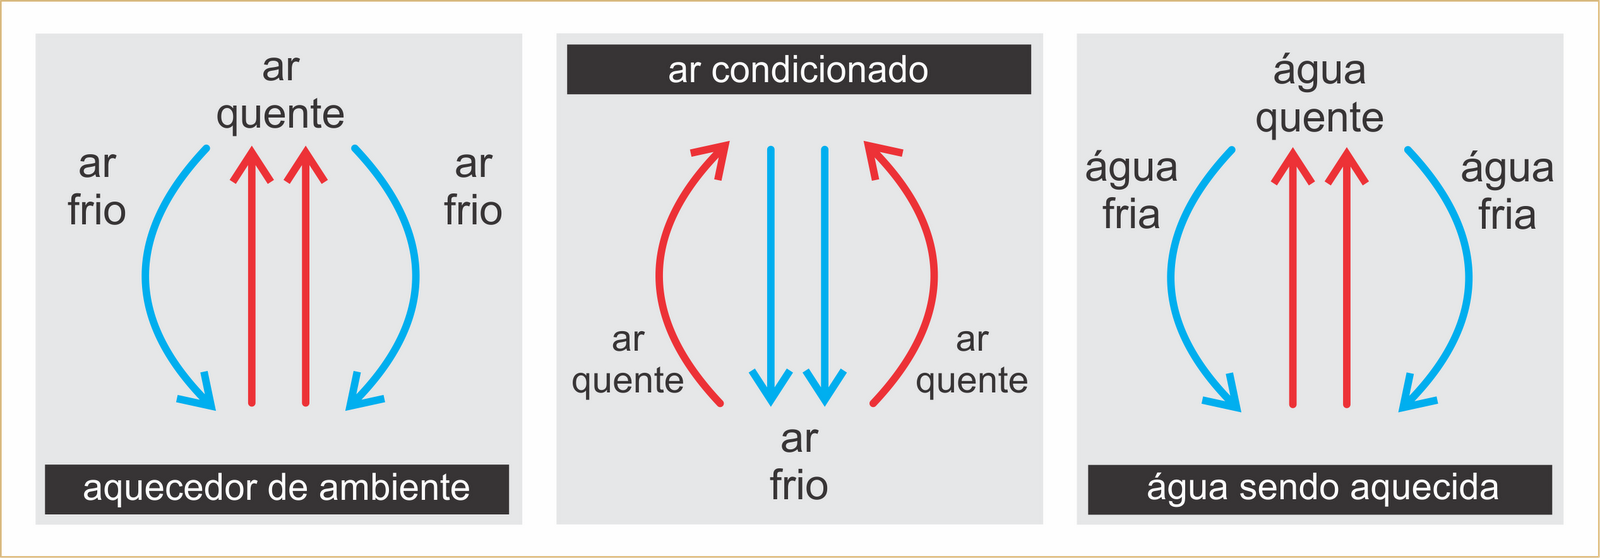
\includegraphics[width=2.5truein]{conveccao.png}
\caption{Correntes de convecção. Fonte: blog os fundamentos da física}

\end{figure}

Confira alguns exemplos:


\begin{itemize}

\item Os aquecedores são instalados próximos ao piso dos cômodos já que a densidade do ar quente é menor que a densidade do ar frio, fazendo com que o ar que sai do aquecedor suba, elevando a temperatura de todo o cômodo.

\item O ar condicionado é instalado no alto, desse modo, o ar frio que ele injeta no interior no ambiente tende a descer, graças à sua densidade.

\item Os exaustores, comuns em mercados e galpões, são usados para que o ar quente que sobe possa circular para o exterior das construções, mantendo-as resfriadas.

\item O material magmático (lava) move-se no interior do manto terrestre e é expelido pelos vulcões, devido às correntes de convecção.

\item A radiação solar evapora a água, esse vapor sobe e condensa-se ao atingir grandes altitudes, dando origem a nuvens de chuva.

\end{itemize}


\textbf{Exercício Resolvido 4}


O calor específico da água é maior do que o calor específico da areia. Assim, durante o dia, numa região litorânea, a areia se aquece mais do que a água do mar. O ar aquecido acima da areia sobe e produz uma região de baixa pressão, aspirando o ar sobre o mar. Sopra a brisa marítima. Explique por que à noite o processo se inverte, isto é, sopra a brisa terrestre?


\begin{figure}[h]{}
\centering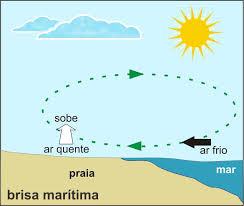
\includegraphics[width=2.5truein]{praia2.jpg}
\caption{Inversão térmica. Fonte: professor Nelson Reys}

\end{figure}

\begin{resposta*}
{\it A água, tendo alto calor específico, sofre variações de temperatura relativamente pequenas. Sendo assim, numa região litorânea, a areia se aquece mais do que o mar durante o dia. O ar aquecido, em contato com a areia, sobe e produz uma região de baixa pressão, aspirando o ar que está sobre o mar. Sopra a brisa marítima. À noite, ao perder calor, a areia se resfria mais do que o mar. O processo se inverte e sopra a brisa terrestre.}
\end{resposta*}

\hypertarget{x-irradiação}{\section{Irradiação}}
Já processo de transmissão de energia por meio de \textbf{ondas eletromagnéticas} é denominada \textbf{irradiação} ou \textbf{radiação}. Quando estas ondas são \textbf{raios infravermelhos}, estamos falando de \textbf{irradiação térmica}.


Ao contrário da condução e da convecção, a irradiação \textbf{não necessita} de meio material: o tranporte é exclusivamente em forma de \textbf{energia}, sob formas de \textbf{ondas}.


Quando a energia radiante incide na superfície de um corpo (\textbf{$Q_{i}$}), ela é parcialmente absorvida (\textbf{$Q_{a}$}), refletida (\textbf{$Q_{r}$}) e transmitida (\textbf{$Q_{t}$}), de modo que: \[Q_{i}=Q_{a}+Q_{r}+Q_{t}\]


\begin{figure}[ht]{}
\centering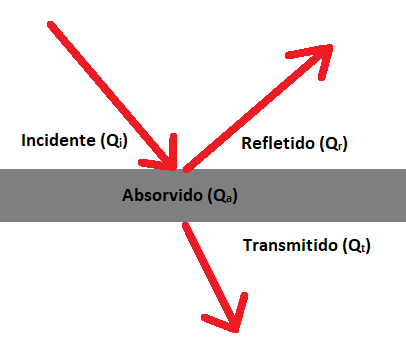
\includegraphics[width=2.5truein]{placa.png}
\caption{Incidencia de calor em uma placa. Fonte: o autor}

\end{figure}

Assim, podemos definir as seguintes grandezas \textbf{adimensionais}:


\textbf{Absorvidade}:\[\boxed{a=\dfrac{Q_{a}}{Q_{i}}}\]


\textbf{Refletividade}:\[\boxed{r=\dfrac{Q_{r}}{Q_{i}}}\]


\textbf{Transmissividade}:\[\boxed{t=\dfrac{Q_{t}}{Q_{i}}}\]


Somando estas três grandezas, temos:


\begin{align*}
a+r+t &=\dfrac{Q_{a}}{Q_{i}} + \dfrac{Q_{r}}{Q_{i}} + \dfrac{Q_{t}}{Q_{i}} \\
&=\dfrac{Q_{a}+Q_{r}+Q_{t}}{Q_{i}} \\
&=\dfrac{Q_{i}}{Q_{i}} \\
&=1
\end{align*}


Ou seja, \[\boxed{a+r+t=1}\]


\textbf{Exercício Resolvido 5}


A quantidade de calor incidente em uma película insulfilm num determinado carro é igual $8\times 10^{3}\;J$. Ela absorve $6\times 10^{3}\;J$ e reflete $1\times 10^3\;J$. Determine a) a absorvidade, b) a reflexividade e c) a transmissividade desta película.


\begin{resposta*}
{\it a) Utilizando a fórmula da absorvidade:
\begin{align*}
a &= \dfrac{Q_{a}}{Q_{i}} \\
&=\dfrac{6\times 10^{3}}{8\times 10^{3}} \\
&={0,75}
\end{align*}
Ou seja, $\boxed{75\%}$ da quantidade de calor é absorvida pela película. \\
b) Utilizando a fórmula da reflexividade:
\begin{align*}
r &= \dfrac{Q_{r}}{Q_{i}} \\
&=\dfrac{1\times 10^{3}}{8\times 10^{3}} \\
&={0,125}
\end{align*}
Ou seja, $\boxed{12,5\%}$ da quantidade de calor é refletida pela película. \\
c) Utilizando a relação entre absorvidade, reflexividade e transmissividade, temos:
\begin{align*}
a+r+t &=1 \\
0,75+0,125+t &= 1 \\
t&=1-0,75-0,125 \\
t&=0,125
\end{align*}
Ou seja, $\boxed{12,5\%}$ da quantidade de calor também é transmitida pela película.}
\end{resposta*}

Quando não há transmissão de energia radiante através do corpo, a transmissividade é nula (\textbf{$t=0$}), neste caso: \[\boxed{a+r=1}\]


Sendo assim, podemos definir um \textbf{corpo negro} como um corpo ideal que \textbf{absorve toda a energia radiante incidente}. Daí a sua absorvidade \textbf{$a=1$ ($100\%$)} e sua reflexidade é nula \textbf{($r=0$)}. O \textbf{espelho ideal} é um corpo que \textbf{reflete totalmente a energia radiante que nele incide}, tendo absorvidade nula (\textbf{$a=0$}) e reflexividade \textbf{$r=1$ ($100\%$)}.


Em geral, os \textbf{corpos escuros} apresentam absorvidade elevada e reflexividade baixa, sendo \textbf{bons absorvedores}. Ao contrário, os \textbf{corpos claros} são \textbf{maus absorvedores}.


\textbf{Corpo negro}:
\begin{align*}
a &= 1\\
r &= 0
\end{align*}


\textbf{Espelho ideal}:
\begin{align*}
a &= 0\\
r &= 1
\end{align*}


Em \textbf{equilíbrio térmico}, um corpo \textbf{polido (alta reflexividade)}, \textbf{absorverá pouca energia}, e assim \textbf{emitindo pouca energia} também. Enquanto um \textbf{corpo escuro (alta absorvidade)}, \textbf{absorverá grande quantidade de energia} e, portanto, \textbf{emitirá também grande quantidade de energia}.


Sendo assim, \textbf{todo} corpo bom absorvedor é bom emissor e todo corpo com refletor é mau emissor. Um \textbf{corpo negro}, sendo um \textbf{absorvedor ideal}, é também um \textbf{emissor ideal ou perfeito}.


\hypertarget{x-lei-de-stefan-boltzmann}{\subsection{Lei de Stefan-Boltzmann}}
Bem, por enquanto está tranquilo, não mesmo? Então, agora vamos estudar uma Lei que tem uma relação direta com a \textbf{Física Moderna}, irei apresentar agora alguns conceitos e fórmulas um pouco mais complexos, mas tenho certeza que você \textbf{tem toda capacidade de aprender}. Então, respira, toma um café, porque iremos estudar agora a \textbf{Lei de Stefan-Boltzmann}.


Podemos definir o \textbf{poder emissivo ($E$)} de um corpo é a \textbf{potência ($P$) irradiada (emitida) por unidade de área ($A$)}, matematicamente: \[E=\dfrac{P}{A}\]


As unidades usuais do poder emissivo são: \textbf{$W/m^{2}$} e \textbf{$cal/(s.cm^{2})$}. Esta grandeza depende da \textbf{natureza} e da \textbf{temperatura} no qual o corpo se encontra. Para cada temperatura, o \textbf{maior poder emissivo é o do corpo negro}, sendo seu valor estabelecido pela Lei de Stefan-Boltzmann: \textbf{o poder emissivo do corpo negro ($E_{cn}$}) é proporcional à \textbf{quarta potência} da sua \textbf{temperatura absoluta ($T$)}. \[E_{cn}=\sigma \cdot T^{4}\]


A constante de proporcionalidade $\sigma$ (\textbf{constante de Stefan-Boltzmann}) vale, em unidade do Sistema Internacional (\textbf{SI}): \[\sigma=5,67\times 10^{-8}\; \dfrac{W}{m^{2}\cdot K^{4}}\]


É comum compararmos o poder emissivo (\textbf{$E$}) de um corpo qualquer com o do corpo negro (\textbf{$E_{cn}$}), por meio de uma grandeza denominada \textbf{emissividade (e)}: \[e=\dfrac{E}{E_{cn}}\]


Evidentemente, o corpo negro apresenta uma emissividade unitária, ou seja: \textbf{$e_{cn}=1$}.


Sendo assim, para \textbf{qualquer corpo}, a lei de Stefan-Bolzmann pode ser escrita algebricamente da seguinte maneira: \[E=e\cdot \sigma \cdot T^{4}\].


Você pode perceber que, o corpo negro tem \textbf{absorvidade $a_{cn}=1$ e emissividade $e_{cn}=1$ ($a_{cn}=e_{cn}$)}. Para qualquer corpo, Kirchoff estabeleceu que: \textbf{$e=a$}. Isto é: \textbf{numa mesma temperatura, a emissividade e a absorvidade de um corpo são iguais}.


Isso vem a confirmar que \textbf{um bom absorvedor de calor também é um bom emissor}.


\textbf{Exercício Resolvido 6}


Considere uma grande placa quadrada, de área igual a $33\;m^{2}$, isotérmica, como um corpo negro, mantido a uma temperatura uniforme de $2000\;K$. A potência total associada à emissão deste corpo negro, expressa em $W$, será de aproximadamente: \\
Dados: constante de Stefan−Boltzmann igual a $5,67\times 10^{-8}\;W/(m^{2}\cdot K^{4})$.


a) $1\times 10^{7}$. \\
b) $2\times 10^{7}$. \\
c) $3\times 10^{7}$. \\
d) $4\times 10^{7}$. \\
c) $5\times 10^{7}$.


\begin{resposta*}
{\it Primeiramente, vamos utilizar a Lei de Stefan-Boltzmann para calcular o poder emissivo deste corpo:
\begin{align*}
E &= \sigma \cdot T^{4} \\
E &= 5,67\times 10^{-8} \cdot (2000)^{4} \\
E &= 5,67\times 10^{-8} \cdot 1,6\times 10^{13} \\
E &= 9,072\times 10^{5} \; W/m^{2}
\end{align*}
Agora, utilizando a relação entre poder emissivo e potência emitida:
\begin{align*}
E &= \dfrac{P}{A} \\
P &= E\cdot A \\
P &= 9,072\times 10^{5} \cdot 33 \\
P &\approx 3\times 10^{7}\;W
\end{align*}
Ou seja, uma potência irradiada de aproximadamente: \[\boxed{P \approx 3\times 10^{7}\;W}\]}
\end{resposta*}

A \textbf{potência irradiada ($P$)} por um corpo de \textbf{emissividade (e)}, à \textbf{temperatura (T)} e cuja área exposta ao \textbf{ambiente é (A)}, pode ser expressa, \textbf{matematicamente}, por: \[P=E\cdot A \Rightarrow \boxed{P=e\cdot \sigma \cdot T^{4} \cdot A}\]


Se o corpo está em \textbf{equilíbrio térmico com o ambiente}, sua \textbf{temperatura é constante}. Todavia, se a temperatatura dele e do ambiente forem \textbf{diferentes}, haverá um \textbf{fluxo de energia líquida}. Assim, se o corpo estiver a uma \textbf{temperatura $T$} e o ambiente a uma \textbf{temperatura $T_{a}$}, a \textbf{potência líquida $P_{l}$} de ganho ou perda de energia será dada por: \[\boxed{P_{l} = e \cdot A \cdot \sigma \cdot (T_{a}^{4} - T^{4})}\]


Você pode observar que a \textbf{potência líquida $P_{l}$} será \textbf{positiva} caso o ambiente esteja "mais quente" que o corpo \textbf{($T_{A} > T$)}, isto significa que o corpo está \textbf{recebendo energia}, isto é, \textbf{absorve mais do que emite}. Enquanto que a \textbf{potência líquida ($P_{l}$)} será \textbf{negativa} se o ambiente estiver mais frio que o corpo \textbf{($T_{A} < T$)}, o que significa que o corpo \textbf{perde energia}, isto é, \textbf{emite mais do que absorve}.


\textbf{Exercício Resolvido 7}


Considere que a pele de uma pessoa tenha emissividade de $0,70$ e sua área exposta de $0,27\;m^{2}$. Supondo que a temperatura da pele seja de $37\;°C$ e que o ambiente esteja a $27\;°C$, calcule:


a) o poder emissivo da pele; \\
b) a potência líquida que a pele irradia para o ambiente; \\
c) o módulo da quantidade e energia líquida irradiada peça pele no intervalo de uma hora.


\begin{resposta*}
{\it a) Primeiramente, como precisamos transformar a temperatura da escala Celsius para a escala Kelvin: $T=37+273=310$, temos que: $T=310\;K$.

Com este valor, podemos aplicar na fórmula do poder emissivo de um corpo:
\begin{align*}
E &= e\cdot \sigma \cdot T^{4} \\
E &= 0,70\cdot 5,67\times 10^{-8}\cdot (310)^{4} \\
E &\approx 366,5\;W/m^{2}
\end{align*}

Ou seja, o poder emissivo da pele é igual a: $\boxed{366,5\;W/m^{2}}$. \\

b) Agora, precisamos converter a temperatura do ambiente para kelvin: $T=27+273=300$, daí temos: $T=300\;K$

Aplicando na fórmula da potência líquida irradiada, teremos:
\begin{align*}
P_{l} &= e \cdot A \cdot \sigma \cdot (T_{a}^{4} - T^{4}) \\
P_{l} &= 0,70\cdot 5,67\times 10^{-8}\cdot [(300)^{4} - (310)^{4}] \\
P_{l} &= -12,1\;W
\end{align*}
Ou seja, a potência líquida irradiada pela pele é igual a $\boxed{P_{l}=-12,1\;W}$.

Perceba que o sinal \textbf{negativo} indica que a pele está \textbf{perdendo calor} para o meio ambiente. \\

c) No intervalo de tempo $\Delta t = 1\;h = 3600\;s$, a energia perdida tem módulo dado por:
\begin{align*}
|Q| &= |P_{l}| \cdot \Delta t \\
|Q| &= 12,1 \cdot 3600 \\
|Q| &= 4,36\times 10^{4}\;J\;
\end{align*}
Ou seja, a energia perdida tem módulo igual a: $\boxed{|Q|=4,36\times 10^{4}\;J}$.}
\end{resposta*}

\hypertarget{x-aplicações-e-efeitos-da-radiação}{\subsection{Aplicações e efeitos da radiação}}
\begin{itemize}

\item \textbf{Efeito estufa}: Substâncias presentes na atmosfera terrestre ($CO_{2}$, vapor de água, metano, etc.​) limitam a transferência de calor da Terra para o espaço, durante a noite, mantendo assim um ambiente adequado para a vida. A intensificação desse efeito, devido à ação humana, está provocando o aquecimento global, com graves consequências para o planeta.

\end{itemize}


\begin{figure}[ht]{}
\centering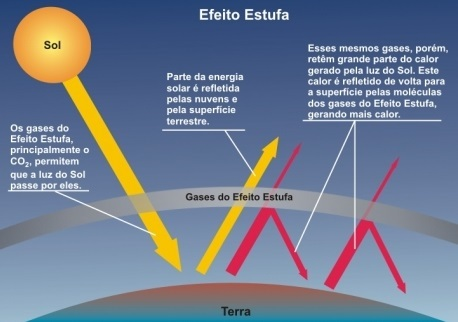
\includegraphics[width=2.5truein]{efeito-estufa2.jpg}
\caption{Efeito estufa. Fonte: professores Juliano e Jacqueline}

\end{figure}

\begin{itemize}

\item \textbf{Garrafa térmica}: Dispositivo no qual são minimizados os três processos de transmissão de calor. O vácuo entre as paredes duplas evita a condução. A boa vedação da garrafa evita a convecção. O espelhamento interno e externo das paredes reduz ao mínimo a irradiação.

\end{itemize}


\begin{figure}[ht]{}
\centering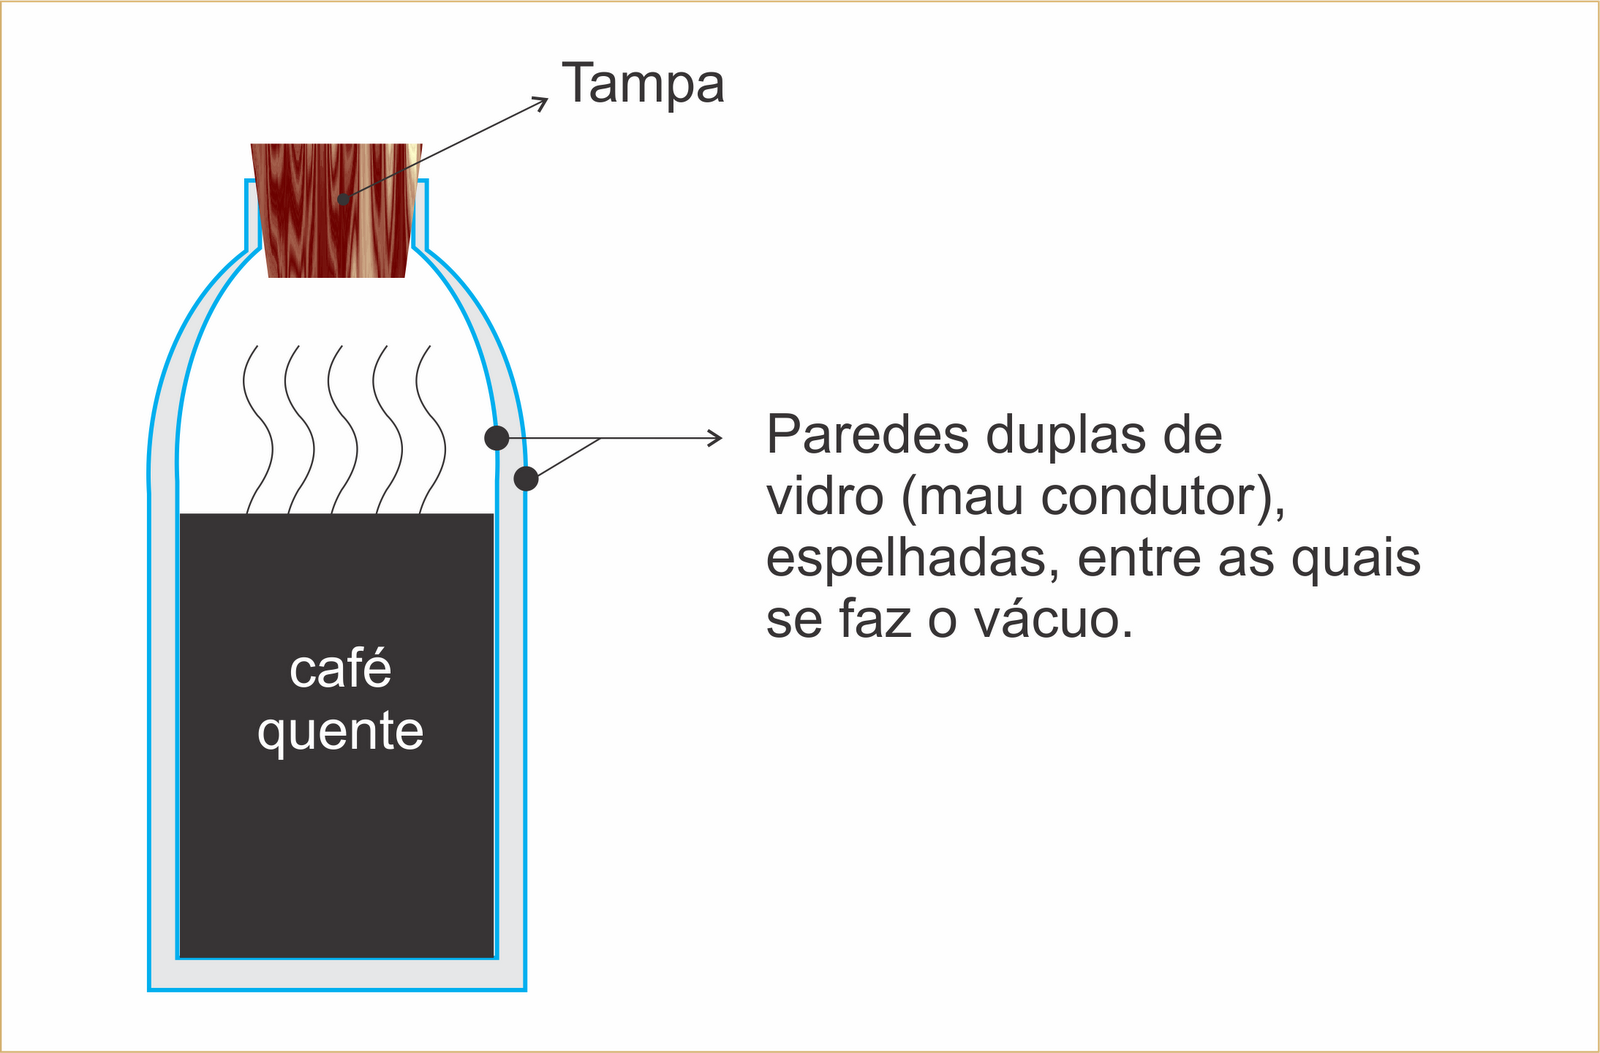
\includegraphics[width=2.5truein]{garrafa-termica.png}
\caption{Garrafa térmica. Fonte: blog os fundamentos da física}

\end{figure}

\hypertarget{x-exercícios-de-revisão}{\section{Exercícios de Revisão}}
1. Uma placa é atravessada por uma quantidade de calor igual a $9,0\times 10^{6}\;cal$ em um intervalo de tempo de $3$ minutos. Determine o fluxo de calor através dessa placa expressa em watt. Considere $1\;cal=4\;J$.


\begin{resposta*}
{\it $5\times 10^{4}\;W$.}
\end{resposta*}

2. \textbf{(UPE)} O fundo de uma panela de alumínio tem espessura $0,30\;cm$ e área de $450\;cm^{2}$. Ao colocá-la sobre uma chama acesa, as temperaturas interna e externa do fundo são de $120\;°C$ e $300\;°C$, respectivamente. Qual o fluxo calorífico através do fundo da panela, sabendo que o coeficiente de condutibilidade do alumínio é $0,05\;cal/(s.cm.°C)$?


a) $10500\;cal/s$. \\
b) $11000\;cal/s$. \\
c) $11500\;cal/s$. \\
d) $12500\;cal/s$. \\
e) $13500\;cal/s$.


\begin{resposta*}
{\it \textbf{e}.}
\end{resposta*}

3. Uma extremidade de uma barra de ferro está em contato com vapor de água em ebulição sob pressão normal ($100\;°C$). A outra extremidade está em contato com gelo em fusão sob pressão normal ($0\;°C$).


A barra tem comprimento L e área de seção reta A. Despreze o calor perdido pela superfície lateral. Seja $\phi_{1}$ o fluxo de calor que atravessa a barra.


Corta-se a barra ao meio e os dois pedaços são soldados. Mantém-se as extremidades às temperaturas de $100\;°C$ e $0\;°C$. Seja $\phi_{2}$ o fluxo de calor que atravessa o novo sistema assim formado. Qual é a razão entre $\phi_{1}$ e $\phi_{2}$?


\begin{figure}[ht]{}
\centering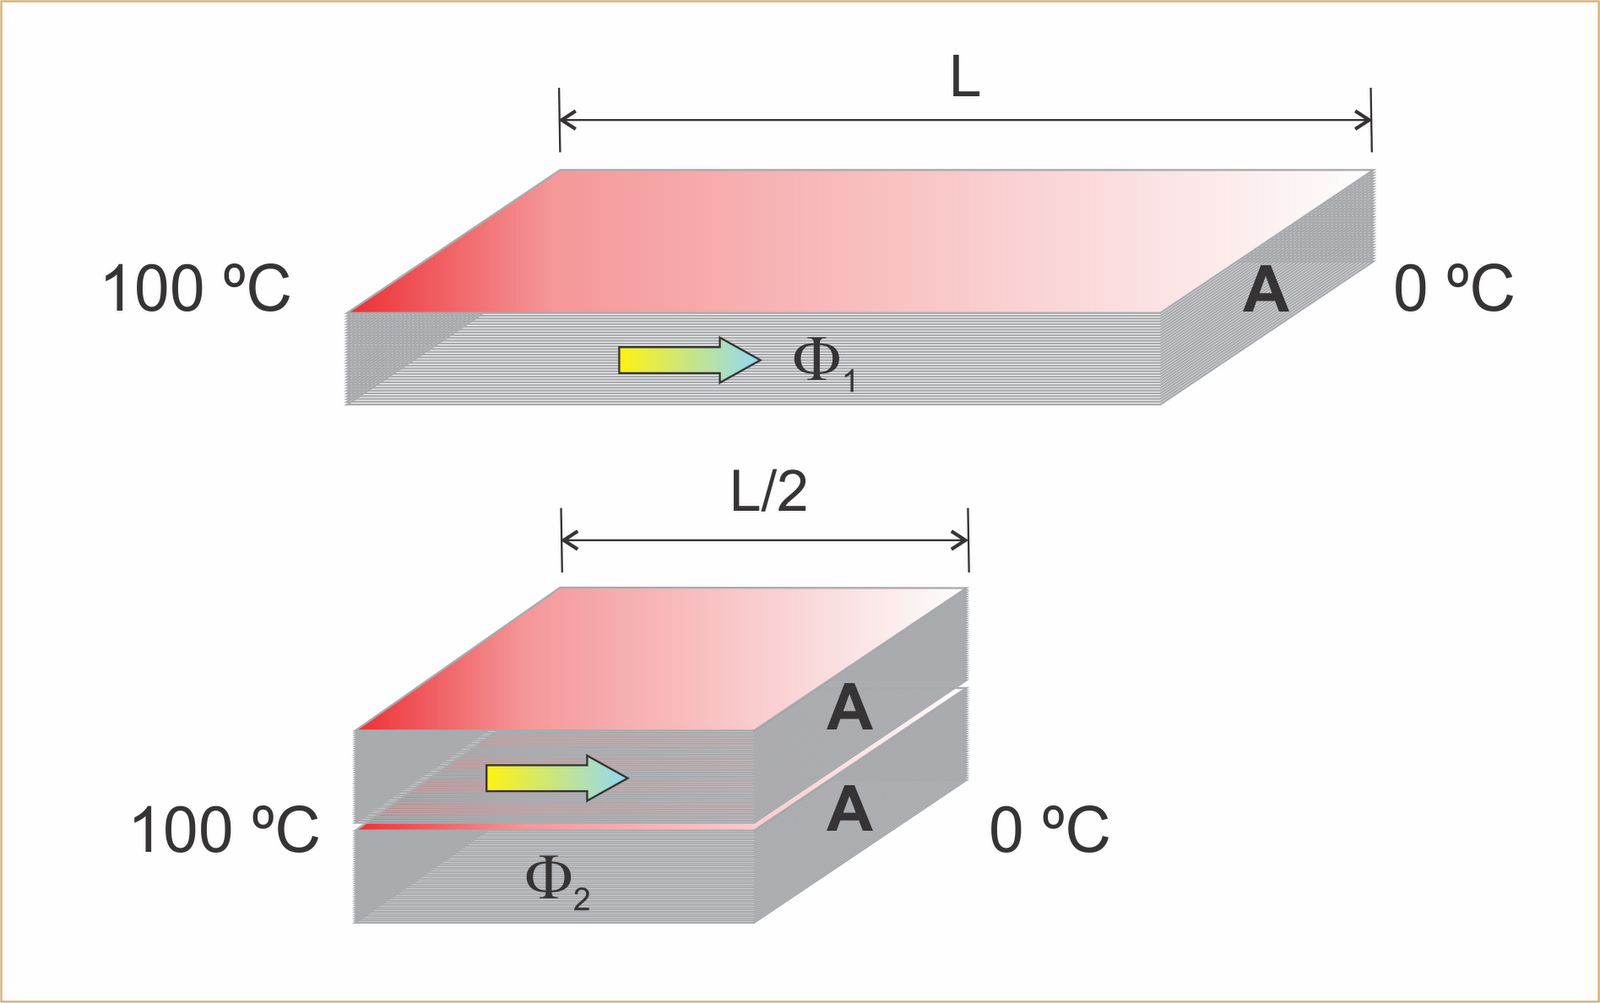
\includegraphics[width=2.5truein]{exerev-img1.png}
\caption{Barra. Fonte: blog os fundamentos da física}

\end{figure}

\begin{resposta*}
{\it $1/4$.}
\end{resposta*}

4. Duas barras de mesmo comprimento, mesma área de seção reta e constituídas de metais diferentes são soldadas e suas outras extremidades mantidas às temperaturas $100\;°C$ e $0\;°C$. Despreze a perda de calor pela superfície lateral. Os coeficientes de condutibilidade térmica dos metais que constituem as barras do sistema são $K_{1}$ e $K_{2}$. A temperatura da junção é de $40\;°C$. Qual é a relação entre $K_{1}$ e $K_{2}$?


\begin{figure}[ht]{}
\centering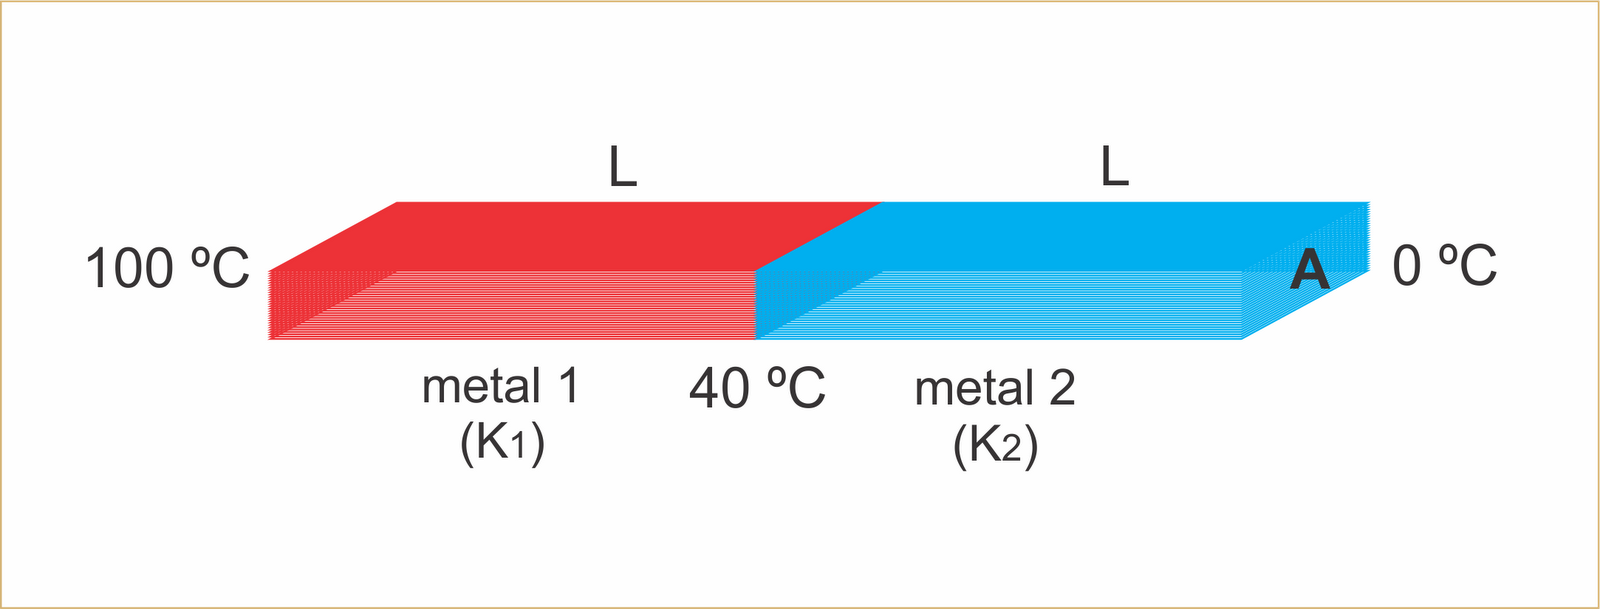
\includegraphics[width=2.5truein]{exerev-img2.png}
\caption{Duas placas. Fonte: blog os fundamentos da física}

\end{figure}

\begin{resposta*}
{\it $2/3$.}
\end{resposta*}

5. A seguir são feitas três afirmações sobre processos termodinâmicos envolvendo transferência de energia de um corpo para outro.


I - A radiação é um processo de transferência de energia que não ocorre se os corpos estiverem no vácuo. \\
II - A convecção é um processo de transferência de energia que ocorre em meios fluidos. \\
III - A condução é um processo de transferência de energia que não ocorre se os corpos estiverem à mesma temperatura.


Quais estão corretas?


a) Apenas I. \\
b) Apenas II. \\
c) Apenas III. \\
d) Apenas I e II. \\
e) Apenas II e III.


\begin{resposta*}
{\it \textbf{e}.}
\end{resposta*}

6. Considere as afirmações:


I - A propagação de calor por convecção ocorre nos fluidos em geral. \\
II - A propagação de calor por condução não ocorre no vácuo. \\
III - Uma malha de lã tem como função fornecer calor ao corpo de uma pessoa. \\
IV - O ar atmosférico e o gelo são bons condutores de calor.


Tem-se:


a) Só as afirmações I e II são corretas; \\
b) Só as afirmações III e são corretas; \\
c) Só as afirmações I e III são corretas; \\
d) Só as afirmações I, II e III são corretas; \\
e) Todas as afirmações são corretas.


\begin{resposta*}
{\it \textbf{a}.}
\end{resposta*}

7. \textbf{(ENEM)} A refrigeração e o congelamento de alimentos são responsáveis por uma parte significativa do consumo de energia elétrica numa residência típica. Para diminuir as perdas térmicas de uma geladeira, podem ser tomados alguns cuidados operacionais:


I - Distribuir os alimentos nas prateleiras deixando espaços vazios entre eles, para que ocorra a circulação do ar frio para baixo e do quente para cima. \\
II - Manter as paredes do congelador com camada bem espessa de gelo, para que o aumento da massa de gelo aumente a troca de calor no congelador. \\
III - Limpar o radiador (“grade” na parte de trás) periodicamente, para que a gordura e a poeira que nele se depositam não reduzam a transferência de calor para o ambiente.


Para uma geladeira tradicional é correto indicar, apenas,


a) a operação I. \\
b) a operação II. \\
c) as operações I e II. \\
d) as operações I e III. \\
e) as operações II e III.


\begin{resposta*}
{\it \textbf{d}.}
\end{resposta*}

8. \textbf{(PUC-RS)} Uma garrafa térmica é feita de vidro com face interna espelhada para:


a) reduzir as perdas de calor por radiação. \\
b) reduzir as perdas de calor por convecção. \\
c) reduzir as perdas de calor por condução. \\
d) elevar o ponto de ebulição da água. \\
e) impedir a formação de vapor de água.


\begin{resposta*}
{\it \textbf{a}.}
\end{resposta*}

9. Uma placa quadrada de $2\;m^{2}$ é irradiada por uma fonte de energia com poder emissivo de $1,6\times 10^{6}\;J/(s.m^{2})$ durante $50$ segundos. Sabendo que esta placa absorve $1\times 10^{8}\;J$ e reflete $2\times 10^{7}\;J$. Determine a) a absorvidade, b) a reflexividade e c) a transmissividade desta placa.


\begin{resposta*}
{\it a) $62,5\%$. \\
b) $12,5\%$. \\
c) $25\%$.}
\end{resposta*}

10. Um objeto de emissividade $0,40$ encontra-se à temperatura de $17\;°C$. A temperatura ambiente é de $37\;°C$. Sendo $0,50\;m^{2}$ sua área exposta, determine:


a) seu poder emissivo; \\
b) a potencia líquida absorvida; \\
c) a quantidade de energia líquida absorvida no intervalo de 10 minutos.


\begin{resposta*}
{\it a) $160,4\;W/m^{2}$. \\
b) $24,5\;W$. \\
c) $1,47\times 10^{4}\;J$.}
\end{resposta*}

11. Numa caixa de vidro de espessura $2,0\;cm$, coloca-se $2,0\;kg$ de gelo. A área da caixa que troca calor com o meio ambiente é de $800\;cm^{2}$. O coeficiente de condutibilidade térmica do vidro é $1,8.10^{-3}$ cal/(cm.s.°C). Qual é a massa de gelo que resta na caixa depois de uma hora, sendo de $0\;°C$ a temperatura interna da caixa e $25\;°C$ a temperatura externa?


Dado: calor específico latente de fusão do gelo: $80\;cal/g$.


\begin{resposta*}
{\it $1190\;g$.}
\end{resposta*}

\hypertarget{x-referências}{\section{Referências}}
FERRARO, Nicolau Gilbert. "Propagação de calor". Blog Os Fundamentos da Física. Disponível em: \href{https://osfundamentosdafisica.blogspot.com/}{https://osfundamentosdafisica.blogspot.com/}


HELERBROCKH, Rafael. "Ponto triplo da água"; Mundo Educação. Disponível em: \href{https://mundoeducacao.uol.com.br/fisica/ponto-triplo-da-agua.htm}{https://mundoeducacao.uol.com.br/fisica/ponto-triplo-da-agua.htm}. Acesso em 02 de agosto de 2020.


HELERBROCKH, Rafael. "Convecção"; Brasil Escola. Disponível em:\\ \href{https://brasilescola.uol.com.br/fisica/conveccao.htm}{https://brasilescola.uol.com.br/fisica/conveccao.htm}. Acesso em 02 de agosto de 2020.


RAMALHO JR, Francisco; FERRARO, Nicolau Gilberto; SOARES, Paulo Antônio de Toledo. Os Fundamentos da Física vol. 2. \textbf{Moderna, São Paulo}, 2007.


VILLAS BÔAS, Newton; DOCA, Ricardo Helou; BISCUOLA, Gualter José. Tópicos de física, 2: termologia, ondulatória e óptica. \textbf{São Paulo: Saraiva}, 2012.


\end{document}

